% !TeX root = scaffold-50.tex
\renewcommand{\imagepath}{../50-unsupervised/img}
\newcommand{\ntopics}{n_\text{topics}}
\newcommand{\nclusters}{n_\text{clusters}}

\chapter{Unsupervised Analysis: Topic Modelling}\label{ch:unsupervised}
This chapter covers the unsupervised exploration of topics of the celebrity newspaper articles and their distribution as a function of \gls{ses}, as motivated in chapter~\ref{ch:this_thesis}. It is shown that using \gls{lda} alone for topic modelling does not yield robust and reliable results. In a second approach, the pre-trained Sentence-BERT model in combination with k-means clustering is shown to improve the quality of the topic extraction. The results are then used to examine differences between the distributions of these topics in the low-\gls{ses} and high-\gls{ses} groups. Potential improvements of the approaches, especially for reliably capturing topic connotations, are discussed.

\section{Shortcomings of LDA Topic Modelling}\label{ch:lda_topic_modelling}
In a first attempt, \gls{lda} (see chapter~\ref{ch:lda}) was trained on the corpus of all relevant newspaper articles from the 50-article balanced data set. The balanced dataset was chosen in order to ensure that role models with many articles could not induce a topic bias. The texts were fed to the models in the \textit{noun and verb} stage in order to focus on the meaning-bearing elements of the texts.

Multiple model instances were created, each one parameterized such that it would output a set of $\ntopics$ topics, with $\ntopics$ varied across the model instances. Each of these topics $t$ is defined by a list $T_{\ntopics, t}$ of characterizing topic words.\footnote{In the rest of this chapter, these word lists are always represented as the 10 most significant words. There are, however, many more topic-characterizing words that the \gls{lda} algorithm outputs for each topic.} The model instances were used to estimate the probabilities $p_{i, t}$ that article $i$ would belong to topic $t$. Each newspaper article $i$ was assigned a topic $t_i$ by selecting the topic with the maximum probability:
\begin{align}
    t_i = \arg \max_{t'} p_{i, t'}
\end{align}

Figure~\ref{fig:topic_modelling_schema} illustrates the modelling and assigment process.
\begin{figure}
    \centering
    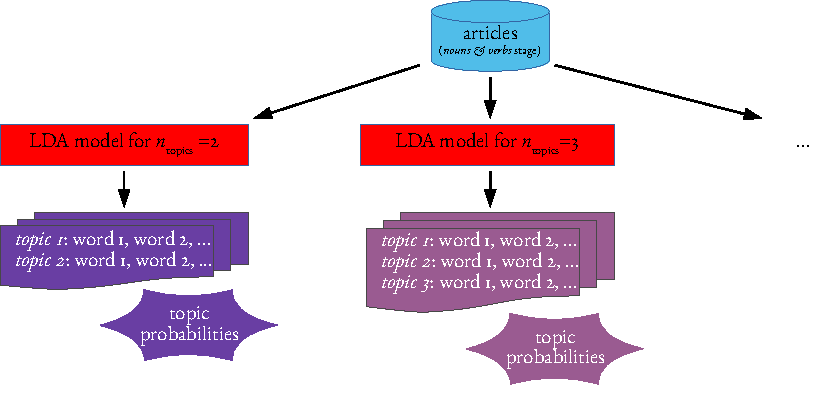
\includegraphics[]{\imagepath/topic_modelling_schema.pdf}
    \caption{Schematic of the topic modelling procedure with \gls{lda}: Many models for different numbers $\ntopics$ of topics are trained, each of them yields a list of topics that are characterized by topic words, as well as topic probabilities for each article.}\label{fig:topic_modelling_schema}
\end{figure}

The \gls{lda} algorithm depends on a set of hyperparameters, most of which are related to its underlying optimization process.  Sensible values for these were found by trial and error. The one hyperparameter that is crucial for the interpretation of this analysis is $\ntopics$. It determines the granularity of the topics the model provides for the comparison of the low- and high-\gls{ses} groups. A trade-off exists between a well-graspable set of topics with considerable overlaps and therefore poor specificity for low $\ntopics$, in contrast to highly delimited niche-topics suffering from a lack of generality for high $\ntopics$. For choosing an appropriate $\ntopics$, it was required that the topics assigned to articles be consistent for small variations of $\ntopics$. Otherwise it could be assumed that the assignment of topics to the articles is to a large part random, which would imply that the findings about the distribution of these topics across the low- and high-\gls{ses} groups are also random. The search for an optimal number of topics included introducing so-called \textit{hypertopics} to make the topics comparable and to identify ranges of $\ntopics$ within which the hypertopic accuracy and the \gls{ses} assignment are consistent:

\paragraph{Assigning Hypertopics}
As the model output topics are only defined by a list of characterizing words, the individual topics can overlap in terms of their meaning (e.g. different kinds of sport), and the topics obtained for different $\ntopics$ cannot be compared without human intuition. In order to still be able to compare the model outputs for different $\ntopics$, each topic was manually assigned one of the four \textit{hypertopics} \textit{movie}, \textit{music}, \textit{sport}, and \textit{life} (with \textit{life} being intended as a miscellaneous category for all topics not covered by the other three hypertopics). These four hypertopics were heuristically selected while examining the model output topics. Each article $i$ with topic $t$ was assigned a hypertopic $h_i$:
\begin{align}
    h_i = h(t_i)
\end{align}
with the manual assignment function $h$ of a hypertopic to a model output topic $t$. Table~\ref{tab:hypertopics_examples} shows examples of the model output topics and their manually assigned hypertopics and shows the generality vs. specificity trade-off in terms of the chosen $\ntopics$.

\begin{table}
    \centering
    \begin{tabular}{clc}
        \toprule
        $\ntopics$ & topic words for exemplary topics (model output) & hypertopic \\
        \toprule 
        \multirow{3}{*}{5} & love video fan people thing song feel music share life & \textit{life}\\
        & game player team season goal win league sport club score & \textit{sport}\\
        & film llc st ave dr series movie season actor michael & \textit{movie}\\
        \midrule
        \multirow{3}{*}{50} & music artist business sony continue record label company team partner & \textit{music} \\
        & inc property water art road town science management development site & \textit{life} \\
        & fc week injury season run football quarter marcel yard dortmund & \textit{sport} \\
        \bottomrule
    \end{tabular}
    \caption{Example of model output topics and their respective hypertopics. Comparing the \textit{sport} hypertopic examples for $\ntopics = 5$ and $\ntopics = 50$ shows how a larger amount of model topics makes the topics more specific, here by referencing a particular sport and a particular sports club.}\label{tab:hypertopics_examples}
\end{table}

With every article associated to a hypertopic, it was possible to compare the distribution of articles and \gls{ses} groups across hypertopics for different $\ntopics$, as well as to verify how accurately the topic models had assigned topics to the articles using the human-annotated data.

\paragraph{Accuracy and Consistency}
The accuracy of the hypertopic assignment was calculated as the ratio of articles with correct hypertopic assignment by the model and all articles that were human-annotated:
\begin{align}\label{eq:accuracy}
    acc = \frac{
        \left|
            \left\{i\middle|h_{i}^\text{predicted} = h_{i}^\text{true}\right\}
        \right|
    }{
        \left|
            \{{i|i \text{ was human-annotated}}\}
        \right|
    }
\end{align}

Figure~\ref{fig:lda_accuracy_diagram} shows that the accuracy varies significantly and inconsistently across $\ntopics$, with a maximum of about \SI{50}{\percent} at $\ntopics=15$.

\begin{figure}
    \centering
    \begin{pgfpicture}
        \pgftext{../../../build/thesis/50-unsupervised/lda_accuracy_diagram.pgf}
    \end{pgfpicture}
    \caption{Accuracy of the model-assigned hypertopics compared to human-annotated data as a function of the number of topics: A maximum accuracy of around \SI{50}{\percent} was achieved for $\ntopics=15$. The accuracy varies significantly across $\ntopics$ and can therefore not be considered consistent.}\label{fig:lda_accuracy_diagram}
\end{figure}

Additionally, the share of low-\gls{ses} articles for each assigned hypertopic was used as a measure for topic assignment consistency across $\ntopics$. This share is plotted in figure~\ref{fig:lda_hypertopic_consistency_diagram}. The fact that there is no range of $\ntopics$ where this share is consistent for small variations of $\ntopics$ suggests that the assignment of articles to the hypertopics is to a considerable extent random and that the model is incapable of making a reliable and consistent prediction of an article's topic. These observations did not differ significantly if the \textit{distinct-\gls{ses}} set of articles was used instead.

\begin{figure}
    \centering
    \begin{pgfpicture}
        \pgftext{../../../build/thesis/50-unsupervised/lda_hypertopic_consistency_diagram.pgf}
    \end{pgfpicture}
    \caption{Share of low-\gls{ses} articles in each hypertopic across different numbers of topics as an indicator of topic assignment consistency: The share varies substantially over a range from \SI{5}{} to \SI{50}{} topics, indicating that the assigment of articles to topics is not very reliable and not consistent. The share of low-\gls{ses} articles among all articles is shown as a reference.}\label{fig:lda_hypertopic_consistency_diagram}
\end{figure}

Two potential approaches for improving accuracy and consistency were examined: Firstly, it was attempted to train the topic models on the low-\gls{ses} and high-\gls{ses} corpora separately, which, however, led to similar inconsistencies. Secondly, it was tried to filter out articles for which the model's topic assignment was ambiguous. As a measure for the ambiguity in topic assignment for article $i$ with topic probabilities $p_{i, t}$, the information theoretical entropy was used~\autocite{gray_entropy_2013}:
\begin{align}
    H_i = -\sum_t p_{i, t} \ln p_{i,t}
\end{align}
The entropy is low if the probability distribution clearly favors a specific topic, and it is high if the probabilities $p_{i, t}$ are rather ambiguous. After filtering out articles where $H_i$ is higher than the \SI{50}{\percent}- or \SI{30}{\percent}-percentile of all articles, higher accuracies of up to \SI{70}{\percent} were reached, however the consistency problem persisted and due to filtering out articles some hypertopics were not present in the remaining set of articles in some cases. The topic modelling quality could hence not be substantially improved by these measures.

The author guesses that one of the reasons for the inconsistent variations in topic assignment is that the newspaper articles have a very limited range of topics, roughly covered by the four hypertopics, which expose considerable overlaps (e.g. movie-related articles having similarity to life stories, film music-related articles talking about movies). This could render the topic models incapable of capturing distinct groups of articles, rather than assigning topics seemingly at random.

As the quality of the topic modelling approach could not be substantially improved within the scope of \gls{lda}, the modelling process was enhanced by adding a pre-trained transformer model as described in the next section.

\section{Improvement with a Pre-Trained Model}\label{ch:pretrained_topic_modelling}
In order to mitigate the issue that the \gls{lda} topic model was apparently incapable of consistenly separating articles by their meaning, the pre-trained model Sentence-BERT was added to the modelling process. It was used to assign to every newspaper article a context-aware vector representation of its meaning (semantics), that could then be partitioned into topics by a clustering algorithm:

As a first step, each article in the \textit{content} stage, meaning the original article with only minimal cleaning applied, was assigned a $384$ dimensional vector representation by the pre-trained Sentence-BERT model (implemention with \textcite{sbertsentencetransformers_sentencetransformers_nodate}, see chapter~\ref{ch:sentencebert}). As suggested by \textcite{black_using_2020}, these representations were first dimensionality-reduced to \SI{50}{} dimensions using \gls{pca}~\autocite{pearson_liii_1901} and then further reduced to \SI{3}{} dimensions using \gls{tsne}~\autocite{maaten_visualizing_2008}. This procedure yielded a three-dimensional semantic vector representation of each article, such that articles with similar meaning are closer to each other in this vector space than articles with a large difference in meaning.

In the next step, these vectors were then used as inputs for the k-means clustering algorithm~\autocite{macqueen_methods_1967} for partitioning the articles according to their meaning, such that articles with similar meaning are more likely to be within the same cluster whereas articles with differing meaning are more likely to be in different clusters. This algorithm produced $\nclusters$ clusters, each one representing one topic. Figure~\ref{fig:clusters} exemplarily shows the articles' vector representations and the clusters found for $\nclusters=5$ in two dimensions. In this way, the process of assigning topics to each article did not depend on the newspaper article corpus anymore but instead only on the pre-trained Sentence-BERT model.

Finally, \gls{lda} with $\ntopics=1$ was separately applied on the articles of each cluster in the \textit{nouns and verbs} stage, hence with most of the structure removed from the text. In this way, each cluster was assigned a single set of topic words, such that in the end the output of the modelling process had the same structure as for using \gls{lda} alone. In the following, $\ntopics$ and $\nclusters$ are going to be used interchangeably for the effective number of topics that are examined.

Figure~\ref{fig:embedding_modelling_schema} illustrates this modelling procedure from the articles, over the vector representations, to the clusters representing topics.

\begin{figure}
    \centering
    \includegraphics[]{\imagepath/cluster_diagram.pdf}
    \caption{Two-dimensional Sentence-BERT vector representations of the newspaper articles after dimensionality reduction with \gls{pca} and \gls{tsne}. The different colors denote the different clusters found by the k-means algorithm. The clusters may seem to be incontiguous because the clustering was performed on the three-dimensional data whereas this representation is two-dimensional. Note that the two axes have no intuitive meaning, they represent the two main components of the original Sentence-BERT embedding of each article.}\label{fig:clusters}
\end{figure}

\begin{figure}
    \centering
    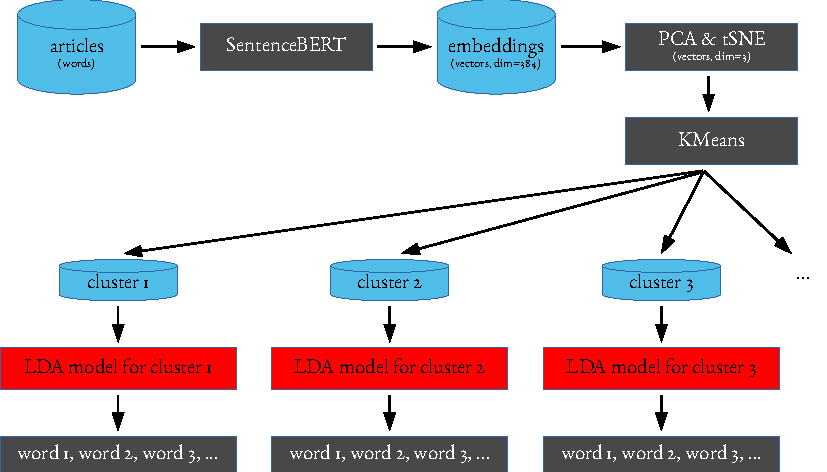
\includegraphics[]{\imagepath/embedding_modelling_schema.pdf}
    \caption{Schematic of the topic modelling process with Sentence-BERT vector representations and k-means clustering: The article texts (in the \textit{content} stage) are transformed into embeddings, a vector representation of text, by the pre-trained Sentence-BERT transformer model. These representations are dimensionality-reduced with \gls{pca} and \gls{tsne}. Then the k-means algorithm clusters the articles into $\nclusters$ clusters. Each of these sets of articles represents a topic whose characterizing words are found by separate \gls{lda} models (with $\ntopics=1$, taking the articles in the \textit{nouns and verbs} stage as input) for each cluster.}\label{fig:embedding_modelling_schema}
\end{figure}

\paragraph{Accuracy and Consistency}
Again, hypertopics were assigned to each set of topic words for evaluating the accuracy and assessing consistency across $\ntopics$. With this enhanced approach, higher accuracies of up to \SI{75}{\percent} and more consistency in topic assignment were achieved, as can be seen from figures~\ref{fig:semantic_clustering_accuracy_diagram} and~\ref{fig:semantic_clustering_hypertopic_consistency_diagram}.

\begin{figure}
    \centering
    %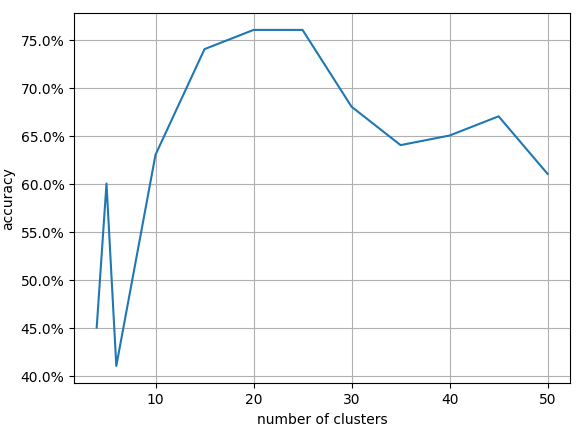
\includegraphics[scale=0.5]{\imagepath/acc_by_n_embeddings.png}
    \begin{pgfpicture}
        \pgftext{../../../build/thesis/50-unsupervised/semantic_clustering_accuracy_diagram.pgf}
    \end{pgfpicture}
    \caption{Accuracy of the pre-trained model-assigned hypertopics compared to human-annotated data as a function of the number of topics: The accuracy is higher and more consistent across the different numbers of clusters compared to the \gls{lda} approach. A value of $\ntopics=20$ seems promising.}\label{fig:semantic_clustering_accuracy_diagram}
\end{figure}

\begin{figure}
    \centering
    % 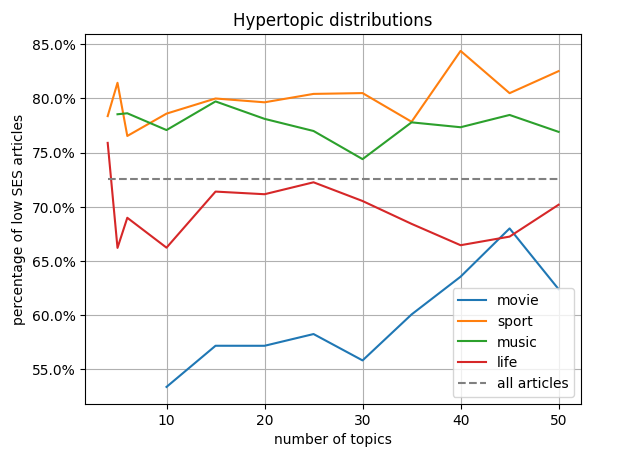
\includegraphics[scale=0.5]{\imagepath/low_ses_by_n_embeddings.png}
    \begin{pgfpicture}
        \pgftext{../../../build/thesis/50-unsupervised/semantic_clustering_hypertopic_consistency_diagram.pgf}
    \end{pgfpicture}
    \caption{Share of low-\gls{ses} articles in each hypertopic across different numbers of topics: The share is comparably consistent around $\ntopics=20$ for all hypertopics, making it a promising choice. The share of low-\gls{ses} articles among all articles is shown as a reference.}\label{fig:semantic_clustering_hypertopic_consistency_diagram}
\end{figure}

As the highest accuracy was achieved for a value of $\ntopics=20$ with comparably little variation around it, this choice was kept for the following analysis. The topic word lists and the assigned hypertopics are listed in the appendix chapter~\ref{ch:unsupervised_appendix} in table~\ref{tab:semantic_clustering_topic_hypertopic_table}. It should be noted that assigning hypertopics was not always unambiguous (see e.g. topics 2 and 7 that could also be \textit{music} instead of \textit{life}). In case of ambiguity, it was decided to label a topic as \textit{life}.

Figure~\ref{fig:embedding_confusion_matrix} compares the hypertopics assigned with the model output and the human-annotated hypertopics. It shows that the overall performance of the model is good at an accuracy of \SI{76}{\percent}, however some of the articles that the human annotator had labelled as \textit{movie} or \textit{music} were subsumed under the hypertopic \textit{life} by the model. This is not surprising considering that celebrity reports do often also cover celebrities' life stories to a significant extent. For the \textit{distinct-SES} approach, somewhat less accuracy is achieved, the predictions appear, however, equally consistent.

\begin{figure}
    \centering
    \includegraphics[]{\imagepath/semantic_clustering_confusion_matrix.pdf}
    \caption{Confusion matrix of the hypertopics for $\ntopics=20$. An accuracy of \SI{76}{\percent} was achieved. The most pronounced difference between the human annotation (``true label'') and the model-based topic assignment (``predicted label'') is that the model subsumes many articles under the \textit{life} hypertopic that the human annotator deems \textit{movie} or \textit{music}.}\label{fig:embedding_confusion_matrix}
\end{figure}

\paragraph{Results}
The distribution of articles across the hypertopics and the \SI{20}{} topics was compared between the low- and high-\gls{ses} groups in order to identify any significant differences in prevalence of topics in the celebrity news coverage between the two \gls{ses} groups. The distribution of the hypertopics for the \textit{mixed-} and the \textit{distinct-SES} approaches is shown in figure~\ref{fig:semantic_clustering_hypertopic_distribution} and listed in table~\ref{tab:embeddings_hypertopics_distribution_and_chi2}. The distribution of all \SI{20}{} topics and their respective topic words is presented in figure~\ref{fig:semantic_clustering_cluster_distribution} the appedix chapter~\ref{ch:unsupervised_appendix}.

\begin{figure}
    \centering
    \begin{subfigure}{0.48\textwidth}
        \centering
        \begin{pgfpicture}
            \pgftext{../../../build/thesis/50-unsupervised/semantic_clustering_hypertopic_distribution.pgf}
        \end{pgfpicture}
        \caption{\textit{mixed-\gls{ses}} approach}
    \end{subfigure}
    \begin{subfigure}{0.48\textwidth}
        \centering
        \begin{pgfpicture}
            \pgftext{../../presentation/img/semantic_clustering_hypertopic_distribution_distinct.pgf}
        \end{pgfpicture}
        \caption{\textit{distinct-\gls{ses}} approach}
    \end{subfigure}
    \caption{Distribution of articles across hypertopics for the low- and the high-\gls{ses} groups; left for the \textit{mixed-}, right for the \textit{distinct-SES} approach. While the \textit{life} hypertopic is equally represented in both \gls{ses} groups, \textit{movie}-related articles prevail more in the high- than in the low-\gls{ses} group, whereas \textit{music} and \textit{sport}-related articles prevail more in the low-\gls{ses} than in the high-\gls{ses} group}\label{fig:semantic_clustering_hypertopic_distribution}
\end{figure}

The graphs reveal that the hypertopic \textit{movie} is more frequent in the high-\gls{ses} group compared to the low-\gls{ses} group, whereas the topics \textit{music} and \textit{sport} are more common in the low-\gls{ses} than in the high-\gls{ses} group. For the all-encompassing \textit{life} hypertopic, the groups show only little difference.

In order to estimate the significance of these differences in the topic distributions, two types of $\chi^2$-tests were performed:
\begin{itemize}
    \item An overall $\chi^2$-contingency test assessed whether it the distribution of articles across topics is different for low- and high-\gls{ses}~\autocite[p. 430]{fahrmeir_spezielle_2016}:
    \begin{align}
        \begin{split}\label{eq:h0_contingency}
            H_{0, \text{contingency}}: ~~~ &\text{distributions } p_{s, t} \text{ over topics } t \text{ are indepedent of } s\\
        & \text{i.e. } p_{s, t} = p_s \cdot p_t ~~ \forall t, s
        \end{split}
    \end{align}
    with the relative frequencies of articles $p_s$ per \gls{ses}, $p_t$ per topic, and $p_{s, t}$ per \gls{ses} and topic. Rejecting $H_{0, \text{contingency}}$ means that the topic distribution can be assumed to be different for low- and high-\gls{ses}.

    \item A second set of $\chi^2$ tests was performed per topic $t$, assessing whether the respective amounts of low- and high-\gls{ses} articles in that topic equals the expected number without dependence on \gls{ses}:
    \begin{align}
        \begin{split}\label{eq:h0_topic}
            H_{0, \text{ topic }t}: ~~~ &\text{number of articles } n_{s, t} \text{ equals expected number } \tilde n_{s, t} \\
            & \text{i.e. } n_{\text{low}, t} = \tilde n_{\text{low}, t} \text{ and } n_{\text{high}, t} = \tilde n_{\text{high}, t}
        \end{split}
    \end{align}
    $\tilde n_{s, t}$ is the expected number of articles per topic under the assumption of an equal percentage of articles in topic $t$ in both \gls{ses} groups:
    \begin{align}
        \tilde n_{s, t} = n_s \cdot \frac{n_t}{n}
    \end{align}
    $n_s$ is the number of articles in \gls{ses} group $s$, $n_t$ the number of articles in topic $t$, and $n$ the total number of articles. Rejecting $H_{0, \text{ topic }t}$ means the prevalence of topic $t$ is not equal in the low- and high-\gls{ses} groups (hence not matching the expectation that topic $t$ would be equally prevailing among the low-\gls{ses} and the high-\gls{ses} articles).
\end{itemize}

Both kinds of $\chi^2$-tests were conducted using the respective functions in the \textit{scipy} library \autocite{scipychi2_scipy_nodate,scipychi2_contingency_scipy_nodate}.

Table~\ref{tab:embeddings_hypertopics_distribution_and_chi2} shows that among the role models mentioned in the survey, newspaper coverage reporting about \textit{music} and \textit{sport} are significantly more common in the low-\gls{ses} group of role models than for the high-\gls{ses} group. On the other hand, newspaper features reporting about \textit{movies} are significantly more frequent in the high-\gls{ses} group of role models than in the low-\gls{ses} group. The \gls{ses} difference in newspaper coverage of ambiguous and other topics, subsumed in the \textit{life} hypertopic, is a lot less pronounced.

\begin{table}
    \centering
    ../../../build/thesis/50-unsupervised/semantic_clustering_hypertopic_chi2_table.tex
    \caption{Distribution of hypertopics for the low- and high-\gls{ses} groups and results of the $\chi^2$-contingency and topic-wise tests. For both the \textit{mixed-} and the \textit{distinct-\gls{ses}} approach, the distributions of topics are significantly different across the \gls{ses} groups. The differences in the hypertopics \textit{movie}, \textit{music}, and \textit{sport} are all significant. It can, however, not be said, that the differences are generally more pronounced for the \textit{distinct-\gls{ses}} approach. Legend: *: $p < \SI{1e-1}{}$, **: $p<\SI{5e-2}{}$, ***: $p<\SI{1e-2}{}$.}\label{tab:embeddings_hypertopics_distribution_and_chi2}
\end{table}

\paragraph{Adjectives and Adverbs}
The topic words of the \textit{nouns and verbs} stage that were output by the model (table~\ref{tab:semantic_clustering_topic_hypertopic_table}) do not expose clear information about connotation and sentiment. Assuming that instead the \textit{adjectives and adverbs} stage could reveal more about the connotations and the sentiment of the newspaper articles, the modelling procedure was modified in order to examine the \textit{adjectives and adverbs} stage of text. To this end, the per-cluster \gls{lda} models were fed with the text in the \textit{adjectives and adverbs} stage instead of the \textit{nouns and verbs} stage. Table \ref{tab:semantic_clustering_adjectives_adverbs_topic_table} in the appendix lists the \SI{20}{} cluster word lists found in this alternative approach. However, these word lists also don't appear to convey any information that could be clearly identified as connotation or sentiment, except for the omnipresent word ``great''. Furthermore, it appears that the part-of-speech tagging didn't work as well as expected since proper names are still among the words, rendering the word lists less interpretable.


\section{Discussion}
In this chapter, topic modelling was explored as a method for analyzing newspaper articles with respect to their topics and their connotation or sentiment. It was shown that \gls{lda} topic modelling alone is outperformed by a modelling approach enhanced by a pre-trained semantic embedding model.

The clearly interpretable results at this stage are unfortunately restricted to the  finding that sports- and music-related topics are comparatively more frequent in the low-\gls{ses} group, whereas movie-related topics are comparatively more frequent in the high-\gls{ses} group. These topics are, however, already well reflected in the professions of the individual role models (see table~\ref{tab:role_model_overview}) and would probably not need a topic modelling approach for identification. To a considerable extent, this is due to the assignment of occupation-related hypertopics. In this first approach, this seems, however, justified as it represented the most straightforward and unambiguous way of subsuming the topics into sensible categories and thereby making model outputs comparable. Also, the adjectives and adverbs describing each topic were unfortunately not indicating any clear connotations.

In order to gain more valuable insights, more sophisticated preprocessing of the data and further enhancing of the modelling procedure will be required. The author deems filtering the training data helpful, e.g. by removing articles whose topic is too closely related to the respective role model's occupation. In this way, the association of role models with their profession wouldn't dominate the topics as much as they do without filtering. In order to facilitate the emergence of sentiment and connotation in the topics, words that don't carry sentiment could be removed from the input fed into the \gls{lda} stages of the modelling process, only leaving connotation- and  sentiment-bearing words in the modelling process. Finally, it could be advisable to examine the model output for high numbers of topics (e.g. $\ntopics>50$) more thoroughly, as in these cases the topics are more specific and could hence expose more connotations in their characterizing word lists.